\documentclass{standalone}
\author{Quinten Bruynseraede}
\usepackage{tikz}
\usetikzlibrary{shapes}
\title{Tikz grafen}
\begin{document}\pagestyle{empty}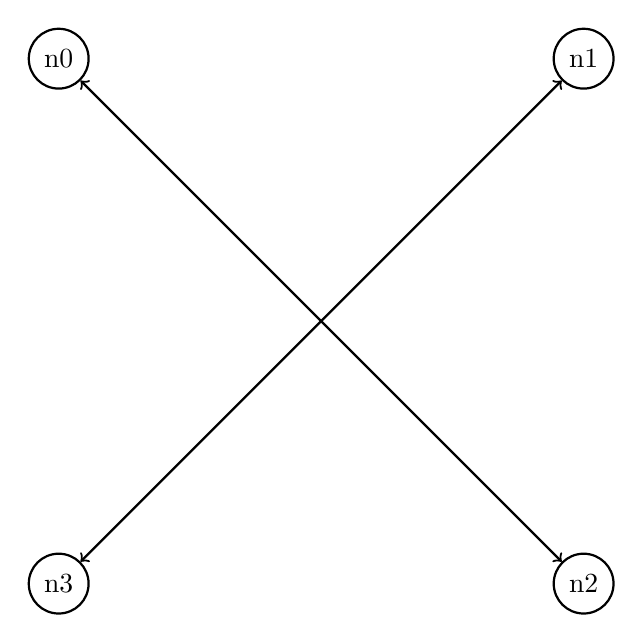
\begin{tikzpicture}\node[shape=circle,draw=black,align=center,line width=0.8pt] (0) at (3.3333333333333335,13.333333333333334) {n0};
\node[shape=circle,draw=black,align=center,line width=0.8pt] (1) at (10.0,13.333333333333334) {n1};
\node[shape=circle,draw=black,align=center,line width=0.8pt] (2) at (3.3333333333333335,6.666666666666667) {n3};
\node[shape=circle,draw=black,align=center,line width=0.8pt] (3) at (10.0,6.666666666666667) {n2};

\path [<->,draw=black,line width=0.8pt] (0) edge node {} (3);
\path [<->,draw=black,line width=0.8pt] (1) edge node {} (2);
\end{tikzpicture}
\end{document}